\section{TMTR}

\begin{frame}{What the paper reports --- TMTR (Fig.~6a)}
\centering
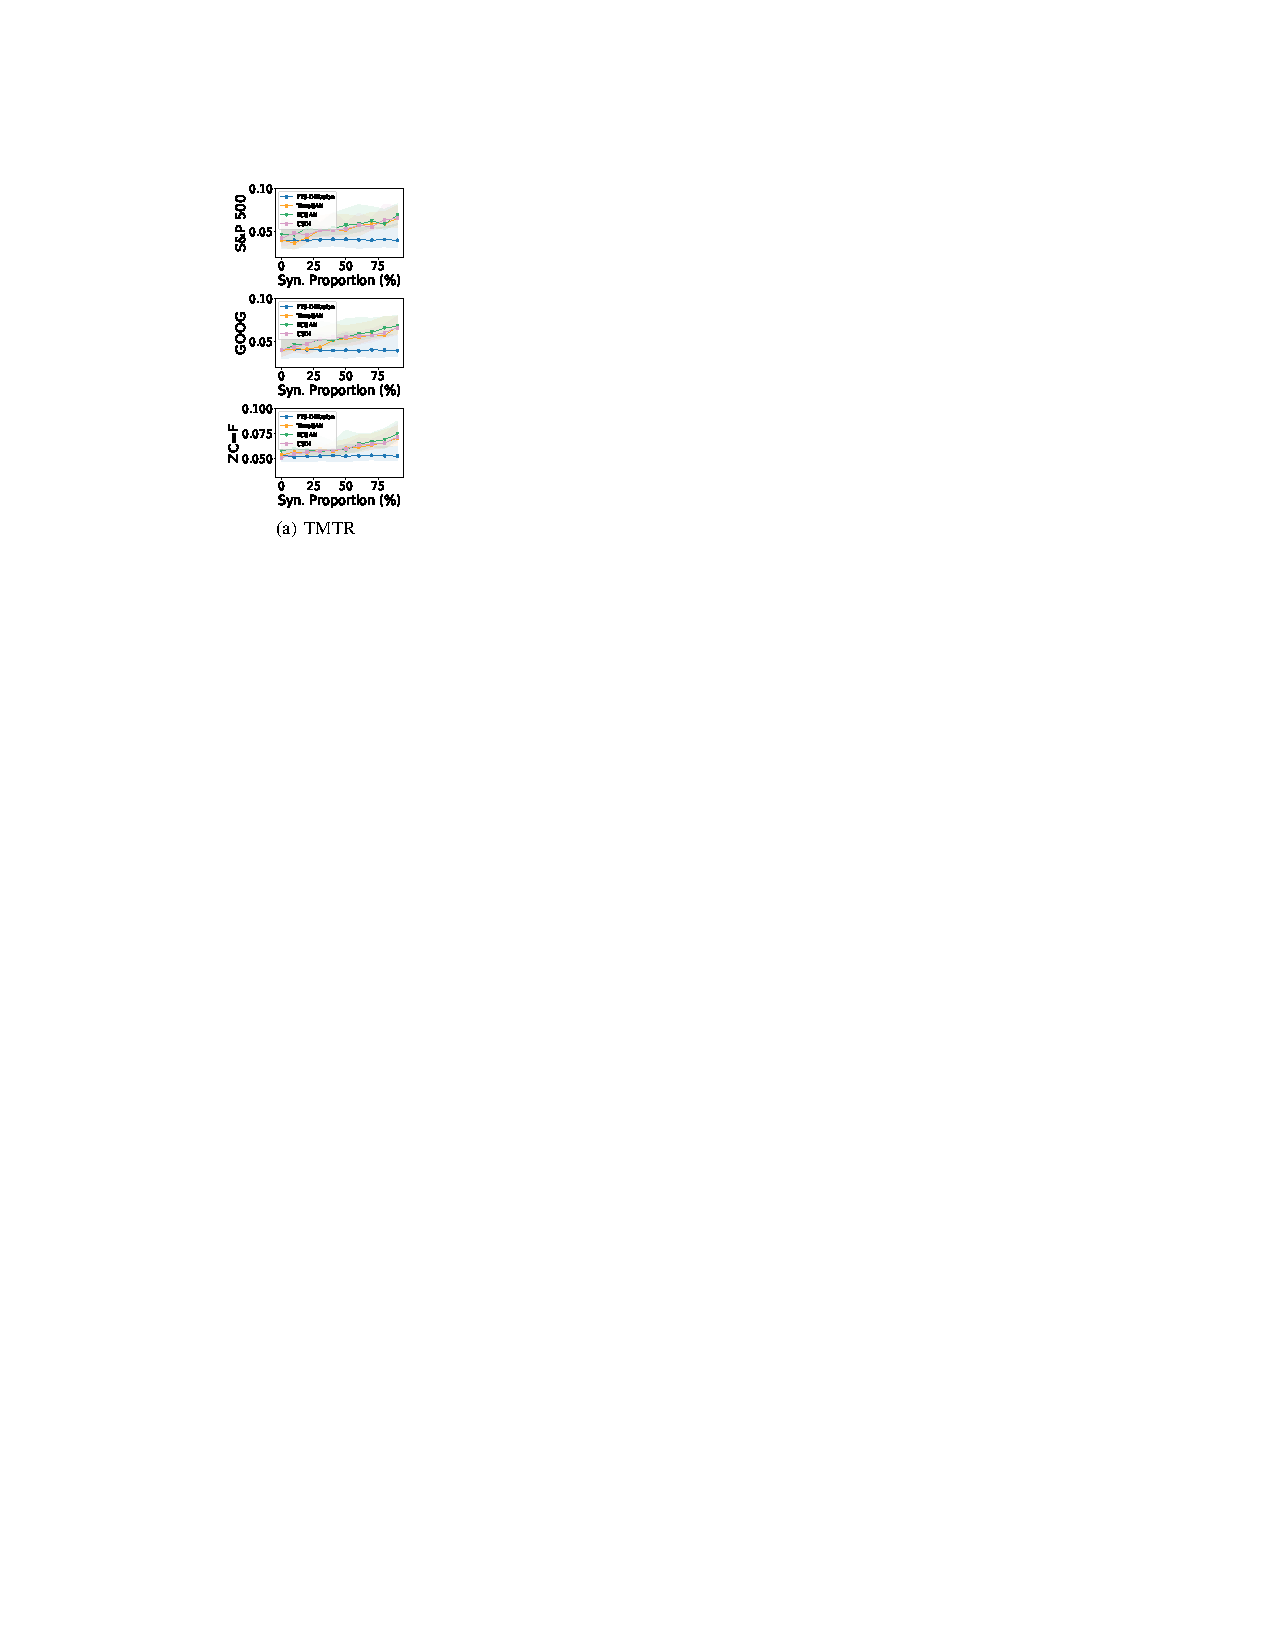
\includegraphics[height=0.74\textheight]{figures/paper/fig6_tmtr.pdf}

\vspace{1mm}
{\footnotesize FTS-Diffusion paper (Yu et al., ICLR 2024), Fig.~6(a): TMTR prediction
error (MAPE) vs.\ synthetic proportion --- FTS-Diffusion vs.\ RCGAN/TimeGAN/CSDI on
S\&P 500, GOOG and ZC$=$F.}
\note{The published TMTR result. FTS-Diffusion keeps MAPE roughly flat as the synthetic proportion rises to 100\%, whereas the baselines degrade --- the paper's evidence that the FTS-Diffusion samples are close enough to real data to substitute for it.}
\end{frame}

\begin{frame}{TMTR: Train on Mixture, Test on Real}

\vspace{4mm}
\centering
\fbox{\parbox[c][5cm][c]{0.78\textwidth}{\centering\itshape figure slot: TMTR per-asset summary}}

% 
\includegraphics[width=0.78\textwidth]{figures/tmtr/sp500/k14/authors/final_enhanced.pdf}
\note{TMTR augments the training set with synthetic FTS-Diffusion samples and evaluates a downstream predictor on the real held-out years. The metric is the same MAPE as in TATR.}
\end{frame}

\begin{frame}{5-day-ahead forecasting}
\begin{alertblock}{Status}
Experiment in progress. No numerical results to report yet.
\end{alertblock}

\vspace{4mm}
\centering
\fbox{\parbox[c][5cm][c]{0.78\textwidth}{\centering\itshape figure slot: 5-day-ahead MAPE / hit-rate}}

% 
\includegraphics[width=0.78\textwidth]{figures/forecast/sp500/k14/authors/final_enhanced.pdf}
\note{Short-horizon forecasting test: use the generative model to roll out 5 future days and compare against the real series. Different metric from TATR (point error rather than distributional).}
\end{frame}
